\documentclass[conference]{IEEEtran}
\IEEEoverridecommandlockouts

\usepackage{cite}
\usepackage{amsmath,amssymb,amsfonts}
\usepackage{algorithmic}
\usepackage{algorithm}
\usepackage{graphicx}
\usepackage{textcomp}
\usepackage{xcolor}
\usepackage{booktabs}
\usepackage{multirow}
\usepackage{url}
\usepackage{balance}

\def\BibTeX{{\rm B\kern-.05em{\sc i\kern-.025em b}\kern-.08em
    T\kern-.1667em\lower.7ex\hbox{E}\kern-.125emX}}

\begin{document}

\title{An Autonomous Multispectral UAV Swarm Framework with Delay-Tolerant Networking and Dual-Threshold Hysteresis EW-CVT for Post-Disaster Search and Rescue}

\author{\IEEEauthorblockN{Devesh Agarwal}
\IEEEauthorblockA{\textit{Department of Computer Science and Engineering} \\
\textit{National Institute of Technology}\\
Email: deveshagarwal652005@gmail.com}
}

\maketitle

\begin{abstract}
Rapid victim localization in post-disaster wilderness and urban debris scenarios presents severe perceptual, communication, and kinetic challenges for autonomous unmanned aerial vehicle (UAV) swarms. Single-modality optical sensors fail in low-contrast conditions, while distributed wireless mesh networks degrade over multi-kilometer operational envelopes due to log-distance path loss and obstacle shadowing. Furthermore, dynamic territorial re-partitioning algorithms, such as Energy-Weighted Centroidal Voronoi Tessellations (EW-CVT), typically suffer from high-frequency trajectory oscillation (chattering) induced by sensor noise and minor centroid drifts, dissipating critical rotor battery energy. In this paper, we propose an end-to-end autonomous multi-UAV search-and-rescue (SAR) framework integrating three tightly coupled innovations: (1) a 4-channel early-fusion multispectral object detector ($640 \times 512 \times 4$, Visible RGB + Thermal LWIR) utilizing a high-resolution P2 stride-4 feature pyramid head to identify small, occluded human targets; (2) a decentralized Flying Ad-Hoc Network (FANET) with an EdgeBroker Delay-Tolerant Networking (DTN) architecture utilizing store-and-forward QoS 1 buffers to guarantee eventual target consensus; and (3) a Dual-Threshold Hysteresis Loop ($\tau_\epsilon = 0.02 \times B_{\text{max}}$, $\tau_\delta = 5.0\,\text{m}$) governing EW-CVT flight commands to eliminate boundary chattering while enforcing an instantaneous hard-override failover trigger upon network topology changes. Validated across large-scale simulations up to $10.24\,\text{km}^2$ and $25\,\text{km}^2$ using real-world multispectral aerial data, the proposed framework achieved $100.0\%$ area survey coverage, $76.83\%$ human victim recall with $3.31\,\text{m}$ localization accuracy, $98.68\%$ chattering suppression saving $24.14\,\text{kJ}$ of propulsion energy, and an energy fairness index of $\mathcal{J} = 0.9998$.
\end{abstract}

\begin{IEEEkeywords}
Autonomous UAV Swarms, Search and Rescue (SAR), Multispectral Early Fusion, Energy-Weighted Voronoi (EW-CVT), Dual-Threshold Hysteresis, Delay-Tolerant Networking (DTN), FANET.
\end{IEEEkeywords}

\section{Introduction}

\subsection{Research Background}
Post-disaster search-and-rescue (SAR) operations following earthquakes, floods, and structural collapses demand immediate, wide-area reconnaissance within the critical ``golden 72 hours'' of survival. Autonomous Unmanned Aerial Vehicle (UAV) swarms offer scalable, rapid-deployment capabilities to survey hazardous, impassable terrains without endangering human responders. However, practical deployment in complex wilderness and disaster debris environments introduces severe cross-layer engineering challenges spanning perception, wireless networking, and spatial flight control.

From a perception standpoint, standard visible-spectrum (RGB) cameras degrade catastrophically under adverse lighting, smoke, shadow occlusion, and camouflage clutter. Long-wave infrared (LWIR) thermal cameras provide robust human signature extraction based on body heat emissivity, yet thermal imagery lacks fine textural and structural edge features. Fusing visible and thermal modalities into a cohesive aerial perception system remains essential for small-target human discovery.

From a networking perspective, Flying Ad-Hoc Networks (FANETs) deployed over multi-kilometer disaster domains suffer from severe radio frequency (RF) attenuation, multipath fading, and non-line-of-sight (NLoS) shadowing caused by mountainous topography and collapsed buildings. Drones operating beyond point-to-point transmission range experience chronic packet dropouts, obstructing real-time swarm coordination and Ground Control Station (GCS) telemetry synchronization.

\subsection{Research Questions}
To achieve reliable autonomous multi-UAV SAR, three fundamental questions must be resolved:
\begin{enumerate}
    \item \textit{How can heterogeneous multispectral sensing be integrated into lightweight edge deep learning architectures to optimize the detection of small, occluded human targets ($<32^2\,\text{px}$) from high-altitude vantage points?}
    \item \textit{How can decentralized swarm consensus and victim alert dissemination be preserved across intermittent, lossy RF mesh networks without overwhelming available wireless channel capacity?}
    \item \textit{How can dynamic, energy-weighted spatial territory partitioning be stabilized to prevent high-frequency trajectory chattering caused by sensor noise and minor centroid migrations, without delaying emergency failover during node crashes?}
\end{enumerate}

\subsection{Research Purpose and Significance}
This research establishes an integrated, mathematically grounded aerial robotics framework addressing these interconnected bottlenecks. By harmonizing a 4-channel early-fusion YOLOv8-P2 perception backbone, a delay-tolerant store-and-forward communication broker, and a dual-threshold hysteresis control loop for Energy-Weighted Centroidal Voronoi Tessellations (EW-CVT), this work eliminates unnecessary propulsion energy waste while providing resilient $100\%$ area coverage. The framework balances energy depletion across surviving swarm agents, ensuring that fatigued drones are not overburdened during in-flight hardware failures.

\subsection{Paper Organization}
The remainder of this paper is organized as follows: Section II reviews related literature in multispectral aerial perception, FANET communications, and Voronoi swarm control. Section III details the mathematical formulation of the proposed system architecture, including the 4-channel detector, RF physics model, EW-CVT partitioning, and the dual-threshold hysteresis loop. Section IV presents empirical results from large-scale simulated SAR missions. Section V concludes the paper with future research directions.

\section{Literature Review}

\subsection{Aerial Multispectral Perception}
Deep learning object detectors, particularly the You Only Look Once (YOLO) family, have become the standard for aerial computer vision. However, standard architectures (YOLOv5 to YOLOv8) employ downsampling strides (8, 16, 32) tailored for medium-to-large objects. Small targets from aerial vantages ($25\text{--}50\,\text{m}$ altitude) frequently collapse within early pooling layers. Recent research has investigated multispectral fusion strategies. Late-fusion ensembles process RGB and thermal feeds through separate backbones before concatenating bounding boxes; however, this doubles computational latency and memory footprints, rendering them impractical for SWaP-constrained (Size, Weight, and Power) edge UAV companions. Early fusion, integrating RGB and thermal channels at the initial convolutional layer, preserves cross-spectral spatial correlations while maintaining near-real-time edge inference speeds.

\subsection{FANETs and Delay-Tolerant Networking}
Communication in multi-UAV swarms relies on decentralized ad-hoc routing. Traditional mobile ad-hoc network (MANET) protocols (e.g., AODV, OLSR) assume continuous, connected topology and fail when inter-UAV distances exceed line-of-sight RF range ($d > 2.5\,\text{km}$). Under disaster conditions, log-distance shadow fading and debris blockage cause frequent network partitioning. Delay-Tolerant Networking (DTN) and store-and-forward architectures buffer undelivered packets in persistent local queues until opportunistic peer proximity enables reliable transmission. However, unconstrained broadcast flooding in DTNs saturates wireless spectrum and causes queue overflow.

\subsection{Voronoi Swarm Partitioning and Flight Stability}
Centroidal Voronoi Tessellations (CVT) and Lloyd's relaxation algorithms partition geographic space by assigning sub-regions based on Euclidean distance to UAV generators. In heterogeneous fleets, Energy-Weighted CVT (EW-CVT) incorporates residual battery capacity into the metric, scaling cell size proportional to available energy. Despite theoretical elegance, standard EW-CVT suffers from high-frequency trajectory chattering: continuous computational ticks subject to Analog-to-Digital Converter (ADC) battery voltage noise and infinitesimal centroid drifts trigger non-stop yaw and roll corrections. This chattering squanders kinetic rotor energy without contributing to search progress.

\subsection{Contributions of This Work}
To address these gaps, our contributions are threefold:
\begin{enumerate}
    \item A unified 4-channel early-fusion YOLOv8n-P2 detector incorporating a stride-4 ($160 \times 128$) P2 head, delivering high recall on small occluded human targets.
    \item An RF physics-informed EdgeBroker communication engine incorporating log-distance shadow fading and store-and-forward QoS 1 buffering, achieving $>80\%$ swarm consensus across partitioned wide-area deployments.
    \item A mathematically formulated Dual-Threshold Hysteresis Loop ($\tau_\epsilon, \tau_\delta$) governing EW-CVT flight commands, suppressing $98.68\%$ of oscillatory turns, saving $24.14\,\text{kJ}$ of rotor energy, and maintaining an instantaneous topology override condition for in-flight motor failover.
\end{enumerate}

\section{System Architecture and Methodology}

The system architecture spans four interconnected layers: Perception, Communication, Spatial Partitioning, and Hysteresis Flight Control, as conceptualized in Fig. 1.

\subsection{4-Channel Early-Fusion Perception (YOLOv8n-P2)}
The perception subsystem ingests calibrated pairs of visible RGB images $\mathbf{I}_{\text{RGB}} \in \mathbb{R}^{H \times W \times 3}$ and Long-Wave Infrared (LWIR) thermal images $\mathbf{I}_{\text{IR}} \in \mathbb{R}^{H \times W \times 1}$. The streams are aligned into a 4-channel multispectral tensor $\mathbf{X} \in \mathbb{R}^{640 \times 512 \times 4}$.

The stem convolution layer is modified to accept four input channels with modified weights $\mathbf{W}_{\text{stem}} \in \mathbb{R}^{C_{\text{out}} \times 4 \times k \times k}$. To resolve small-target feature loss, we introduce a high-resolution P2 feature pyramid head at stride 4. While standard YOLOv8 extracts features at scales P3 ($80 \times 64$), P4 ($40 \times 32$), and P5 ($20 \times 16$), the P2 head fuses low-level spatial geometry directly from layer 2 via path-aggregation feature concatenation:
\begin{equation}
    \mathbf{F}_{\text{P2}} = \text{Conv}\left( \left[ \mathbf{F}_{\text{stem}}^{(2)}, \, \text{Up}_2(\mathbf{F}_{\text{P3}}) \right] \right)
\end{equation}
This yields a high-resolution detection grid of $160 \times 128$ anchor cells, increasing receptive resolution for human targets with ground footprints under $32 \times 32$ pixels.

\subsection{RF Channel Physics and Delay-Tolerant EdgeBroker}
Inter-UAV wireless communication is governed by free-space path loss and log-distance shadow fading over carrier frequency $f = 2.4\,\text{GHz}$ and $5.0\,\text{GHz}$. The total path loss $PL(d)$ at 3D distance $d$ is:
\begin{equation}
    PL(d) = 20 \log_{10}(d) + 20 \log_{10}(f) - 27.55 + X_\sigma
\end{equation}
where $X_\sigma \sim \mathcal{N}(0, \sigma^2)$ is a zero-mean Gaussian random variable representing shadowing clutter ($\sigma = 7.5\,\text{dB}$ for post-disaster debris). The observed Signal-to-Noise Ratio (SNR) at receiver $j$ from transmitter $i$ is:
\begin{equation}
    \text{SNR}_{ij}(d) = P_{\text{tx}} + G_{\text{tx}} + G_{\text{rx}} - PL(d) - P_{\text{noise}}
\end{equation}
where $P_{\text{tx}} = 33\,\text{dBm}\,(2\,\text{W})$, antenna gains $G_{\text{tx}} = G_{\text{rx}} = 2.15\,\text{dBi}$, and thermal noise floor $P_{\text{noise}} = -95\,\text{dBm}$. The dynamic Packet Error Rate (PER) is modeled via a generalized logistic link:
\begin{equation}
    \text{PER}(\text{SNR}) = \frac{1}{1 + \exp\left( k \cdot (\text{SNR} - \text{SNR}_{\text{thresh}}) \right)}
\end{equation}
with $k = 0.5$ and $\text{SNR}_{\text{thresh}} = 10.0\,\text{dB}$.

When $\text{PER}_{ij} > \gamma_{\text{drop}}$, target alert packets $m_k$ are not discarded; rather, the localized EdgeBroker enqueues them into a persistent FIFO QoS 1 buffer:
\begin{equation}
    \mathcal{Q}_i = \left\{ m_k \;\middle|\; \text{SNR}_{ij} < \text{SNR}_{\text{thresh}} \right\}
\end{equation}
When UAVs converge within RF range during criss-crossing search sweeps or Return-to-Launch (RTL) flight at the Ground Control Station, buffers are flushed via high-throughput proximity bursts.

\subsection{Energy-Weighted Centroidal Voronoi Tessellation}
Let $\Omega \subset \mathbb{R}^2$ represent the bounded search arena. The swarm consists of $n$ active UAVs with spatial coordinates $\mathbf{x}_i = (x_i, y_i)$. In standard CVT, cells $V_i$ are assigned via Euclidean distance. Under EW-CVT, the assignment evaluates the power distance weighted by residual battery $B_i(t)$:
\begin{equation}
    d_w(\mathbf{p}, \mathbf{x}_i) = \frac{\|\mathbf{p} - \mathbf{x}_i\|^2}{w_i(t)}
\end{equation}
where the dynamic energy weight $w_i(t)$ is defined as:
\begin{equation}
    w_i(t) = \left( \frac{B_i(t)}{B_{\text{max}}} \right)^\alpha
\end{equation}
Here $\alpha \ge 0$ is the EW-CVT energy weighting sensitivity exponent. The theoretical mass centroid $C_i^*$ of Voronoi cell $V_i$ is computed as:
\begin{equation}
    C_i^* = \frac{\int_{V_i} \mathbf{p} \cdot \rho(\mathbf{p}) \, d\mathbf{p}}{\int_{V_i} \rho(\mathbf{p}) \, d\mathbf{p}}
\end{equation}
where $\rho(\mathbf{p})$ represents a prior spatial victim distribution density.

\subsection{Dual-Threshold Hysteresis Flight Control}
Continuous recalculation of $w_i(t)$ and $C_i^*$ causes high-frequency oscillatory chattering. We introduce a Dual-Threshold Hysteresis Loop that locks updates until kinetic and energy thresholds are exceeded:

\subsubsection{Battery Decay Hysteresis ($\tau_\epsilon$)}
Let $t_k$ denote the timestamp of the last executed partition update. The effective generator weight $w_i(t)$ evaluated at time $t$ is locked unless discharge exceeds margin $\tau_\epsilon$:
\begin{equation}
    w_i(t) = \begin{cases}
        \left( \frac{B_i(t)}{B_{\text{max}}} \right)^\alpha, & \text{if } B_i(t_k) - B_i(t) \ge \tau_\epsilon \\
        w_i(t_k), & \text{otherwise}
    \end{cases}
\end{equation}
where $\tau_\epsilon = 0.02 \times B_{\text{max}}$ (a discrete $2\%$ discharge lock).

\subsubsection{Spatial Centroid Hysteresis ($\tau_\delta$)}
Even after battery discharge, minor adjacent boundary adjustments may shift theoretical centroid $C_i^*$ by only centimeters. Waypoint commands $C_i(t)$ are filtered via:
\begin{equation}
    C_i(t) = \begin{cases}
        C_i^*, & \text{if } \|C_i^* - C_i(t_k)\| \ge \tau_\delta \\
        C_i(t_k), & \text{otherwise}
    \end{cases}
\end{equation}
where $\tau_\delta = 5.0\,\text{m}$, calibrated against UAV turning radius and camera FOV.

\subsubsection{Forced-Override Condition (Node Failure)}
During catastrophic events (e.g., in-flight motor failure), steady-state hysteresis must be bypassed. Let $\mathcal{N}(t)$ denote the active network topology vector derived from Data Link Layer (DLL) heartbeats. The master update trigger $\mathcal{U}_i(t)$ is formulated as:
\begin{equation}
    \mathcal{U}_i(t) = \left( (B_i(t_k) - B_i(t) \ge \tau_\epsilon) \land (\|C_i^* - C_i(t_k)\| \ge \tau_\delta) \right) \lor (\mathcal{N}(t) \ne \mathcal{N}(t_k))
\end{equation}
If $\mathcal{U}_i(t) = \text{True}$, UAV $i$ updates its Voronoi partition, commits baseline $t_k \leftarrow t$, and commands the flight controller. If topology changes ($\mathcal{N}(t) \ne \mathcal{N}(t_k)$), the right-hand term forces an instantaneous hard update, overriding $\tau_\epsilon$ and $\tau_\delta$.

\begin{algorithm}[t]
\caption{Dual-Threshold Hysteresis EW-CVT Flight Control}
\label{alg:hysteresis}
\begin{algorithmic}[1]
\REQUIRE Drone $i$, baseline $(t_k, B_i(t_k), C_i(t_k), \mathcal{N}(t_k))$, thresholds $(\tau_\epsilon, \tau_\delta, \alpha)$
\STATE Read telemetry: current time $t$, battery $B_i(t)$, topology $\mathcal{N}(t)$
\STATE Compute theoretical centroid $C_i^*$ via EW-CVT (Eq. 6--8)
\STATE $\Delta B \leftarrow B_i(t_k) - B_i(t)$
\STATE $\Delta C \leftarrow \|C_i^* - C_i(t_k)\|$
\STATE $\text{topo\_changed} \leftarrow (\mathcal{N}(t) \ne \mathcal{N}(t_k))$
\STATE $\mathcal{U}_i(t) \leftarrow (\Delta B \ge \tau_\epsilon \land \Delta C \ge \tau_\delta) \lor \text{topo\_changed}$
\IF{$\mathcal{U}_i(t)$ is True}
    \STATE $t_k \leftarrow t$, \; $B_i(t_k) \leftarrow B_i(t)$
    \STATE $w_i(t) \leftarrow (B_i(t)/B_{\text{max}})^\alpha$
    \STATE $C_i(t) \leftarrow C_i^*$
    \STATE $\mathcal{N}(t_k) \leftarrow \mathcal{N}(t)$
    \STATE Steer autopilot toward $C_i(t)$
\ELSE
    \STATE Maintain commanded waypoint $C_i(t) \leftarrow C_i(t_k)$
    \STATE Suppress heading jitter; accumulate kinetic energy saved
\ENDIF
\end{algorithmic}
\end{algorithm}

\subsubsection{Kinetic Propulsion Energy Model}
Level flight propulsion power $P_{\text{propulsion}}(v)$ at airspeed $v$ is modeled as:
\begin{equation}
    P_{\text{prop}}(v) = P_0 \left(1 + \frac{3 v^2}{v_{\text{tip}}^2}\right) + P_i \left( \sqrt{1 + \frac{v^4}{4 v_0^4}} - \frac{v^2}{2 v_0^2} \right)^{\frac{1}{2}} + \frac{1}{2} d_0 \rho s A v^3
\end{equation}
The kinetic energy preserved by suppressing a chattering turn is:
\begin{equation}
    E_{\text{saved}} = \frac{1}{2} I_{\text{yaw}} \omega_{\text{yaw}}^2 + \int_0^{\Delta t_{\text{turn}}} P_{\text{prop}}(v) \, dt
\end{equation}

\section{Experimental Evaluation and Analysis}

\subsection{Experimental Setup and Implementation}
The proposed framework was evaluated using the real-world multispectral RGBT DronePerson benchmark dataset, comprising paired visible and thermal aerial frames collected at varying altitudes ($25\text{--}50\,\text{m}$) over disaster-like environments. World sectors were instantiated within the FlyNetSim simulation engine over two extensive footprints:
\begin{itemize}
    \item \textbf{Setup A}: $3200\,\text{m} \times 3200\,\text{m}$ ($10.24\,\text{km}^2$), 6 UAVs, $25$ sectors.
    \item \textbf{Setup B}: $5000\,\text{m} \times 5000\,\text{m}$ ($25.0\,\text{km}^2$), 10 UAVs, injected motor failure on UAV 4 at $T=80\,\text{s}$.
\end{itemize}

All UAVs initiate from a unified Ground Control Station launch pad (SW corner at $5\%$ arena offset). Drones utilize a dual-speed flight envelope: high-speed transit dash at $50\,\text{m/s}$ along non-overlapping radial corridors, decelerating to $32\,\text{m/s}$ optical search cruise upon reaching assigned sectors.

\subsection{Perception Performance Comparison}
We trained the 4-channel YOLOv8n-P2 detector for 40 epochs on dual NVIDIA GPUs and compared it against single-modality baselines (RGB-only, Thermal-only) and the standard YOLOv8n (P3--P5) feature pyramid.

\begin{table}[htbp]
\caption{Multispectral Detection Performance Comparison}
\label{tab:perception}
\centering
\begin{tabular}{lcccc}
\toprule
\textbf{Model \& Modality} & \textbf{Precision} & \textbf{Recall} & \textbf{mAP}$_{50}$ & \textbf{AP}$_S$ ($<32^2\text{px}$) \\
\midrule
YOLOv8n (RGB-only) & 0.412 & 0.528 & 0.463 & 0.214 \\
YOLOv8n (Thermal-only) & 0.447 & 0.589 & 0.512 & 0.268 \\
YOLOv8n (RGB+T Early) & 0.461 & 0.672 & 0.581 & 0.312 \\
\textbf{YOLOv8n-P2 (RGB+T Proposed)} & \textbf{0.481} & \textbf{0.768} & \textbf{0.684} & \textbf{0.429} \\
\bottomrule
\end{tabular}
\end{table}

As documented in Table I, the proposed 4-channel YOLOv8n-P2 achieves a superior recall of $76.83\%$ and boosts small-target average precision ($\text{AP}_S$) by $+37.5\%$ over standard RGB+T YOLOv8n ($0.429$ vs. $0.312$). The stride-4 P2 head retains fine-grained features critical for detecting small human victims under foliage and shadow occlusion.

\subsection{Swarm Spatial Exploration and Network Dynamics}
In Setup A ($10.24\,\text{km}^2$, 6 UAVs), the swarm swept all $25$ sectors within $234\,\text{s}$, achieving $100.0\%$ area survey coverage. The time-to-first-detection (TTFD) was $1.0\,\text{s}$. The swarm identified $199$ verified targets out of $259$ ground-truth human annotations with a mean localization error of $3.31\,\text{m}$ (RMSE $6.87\,\text{m}$).

\begin{figure}[htbp]
\centering
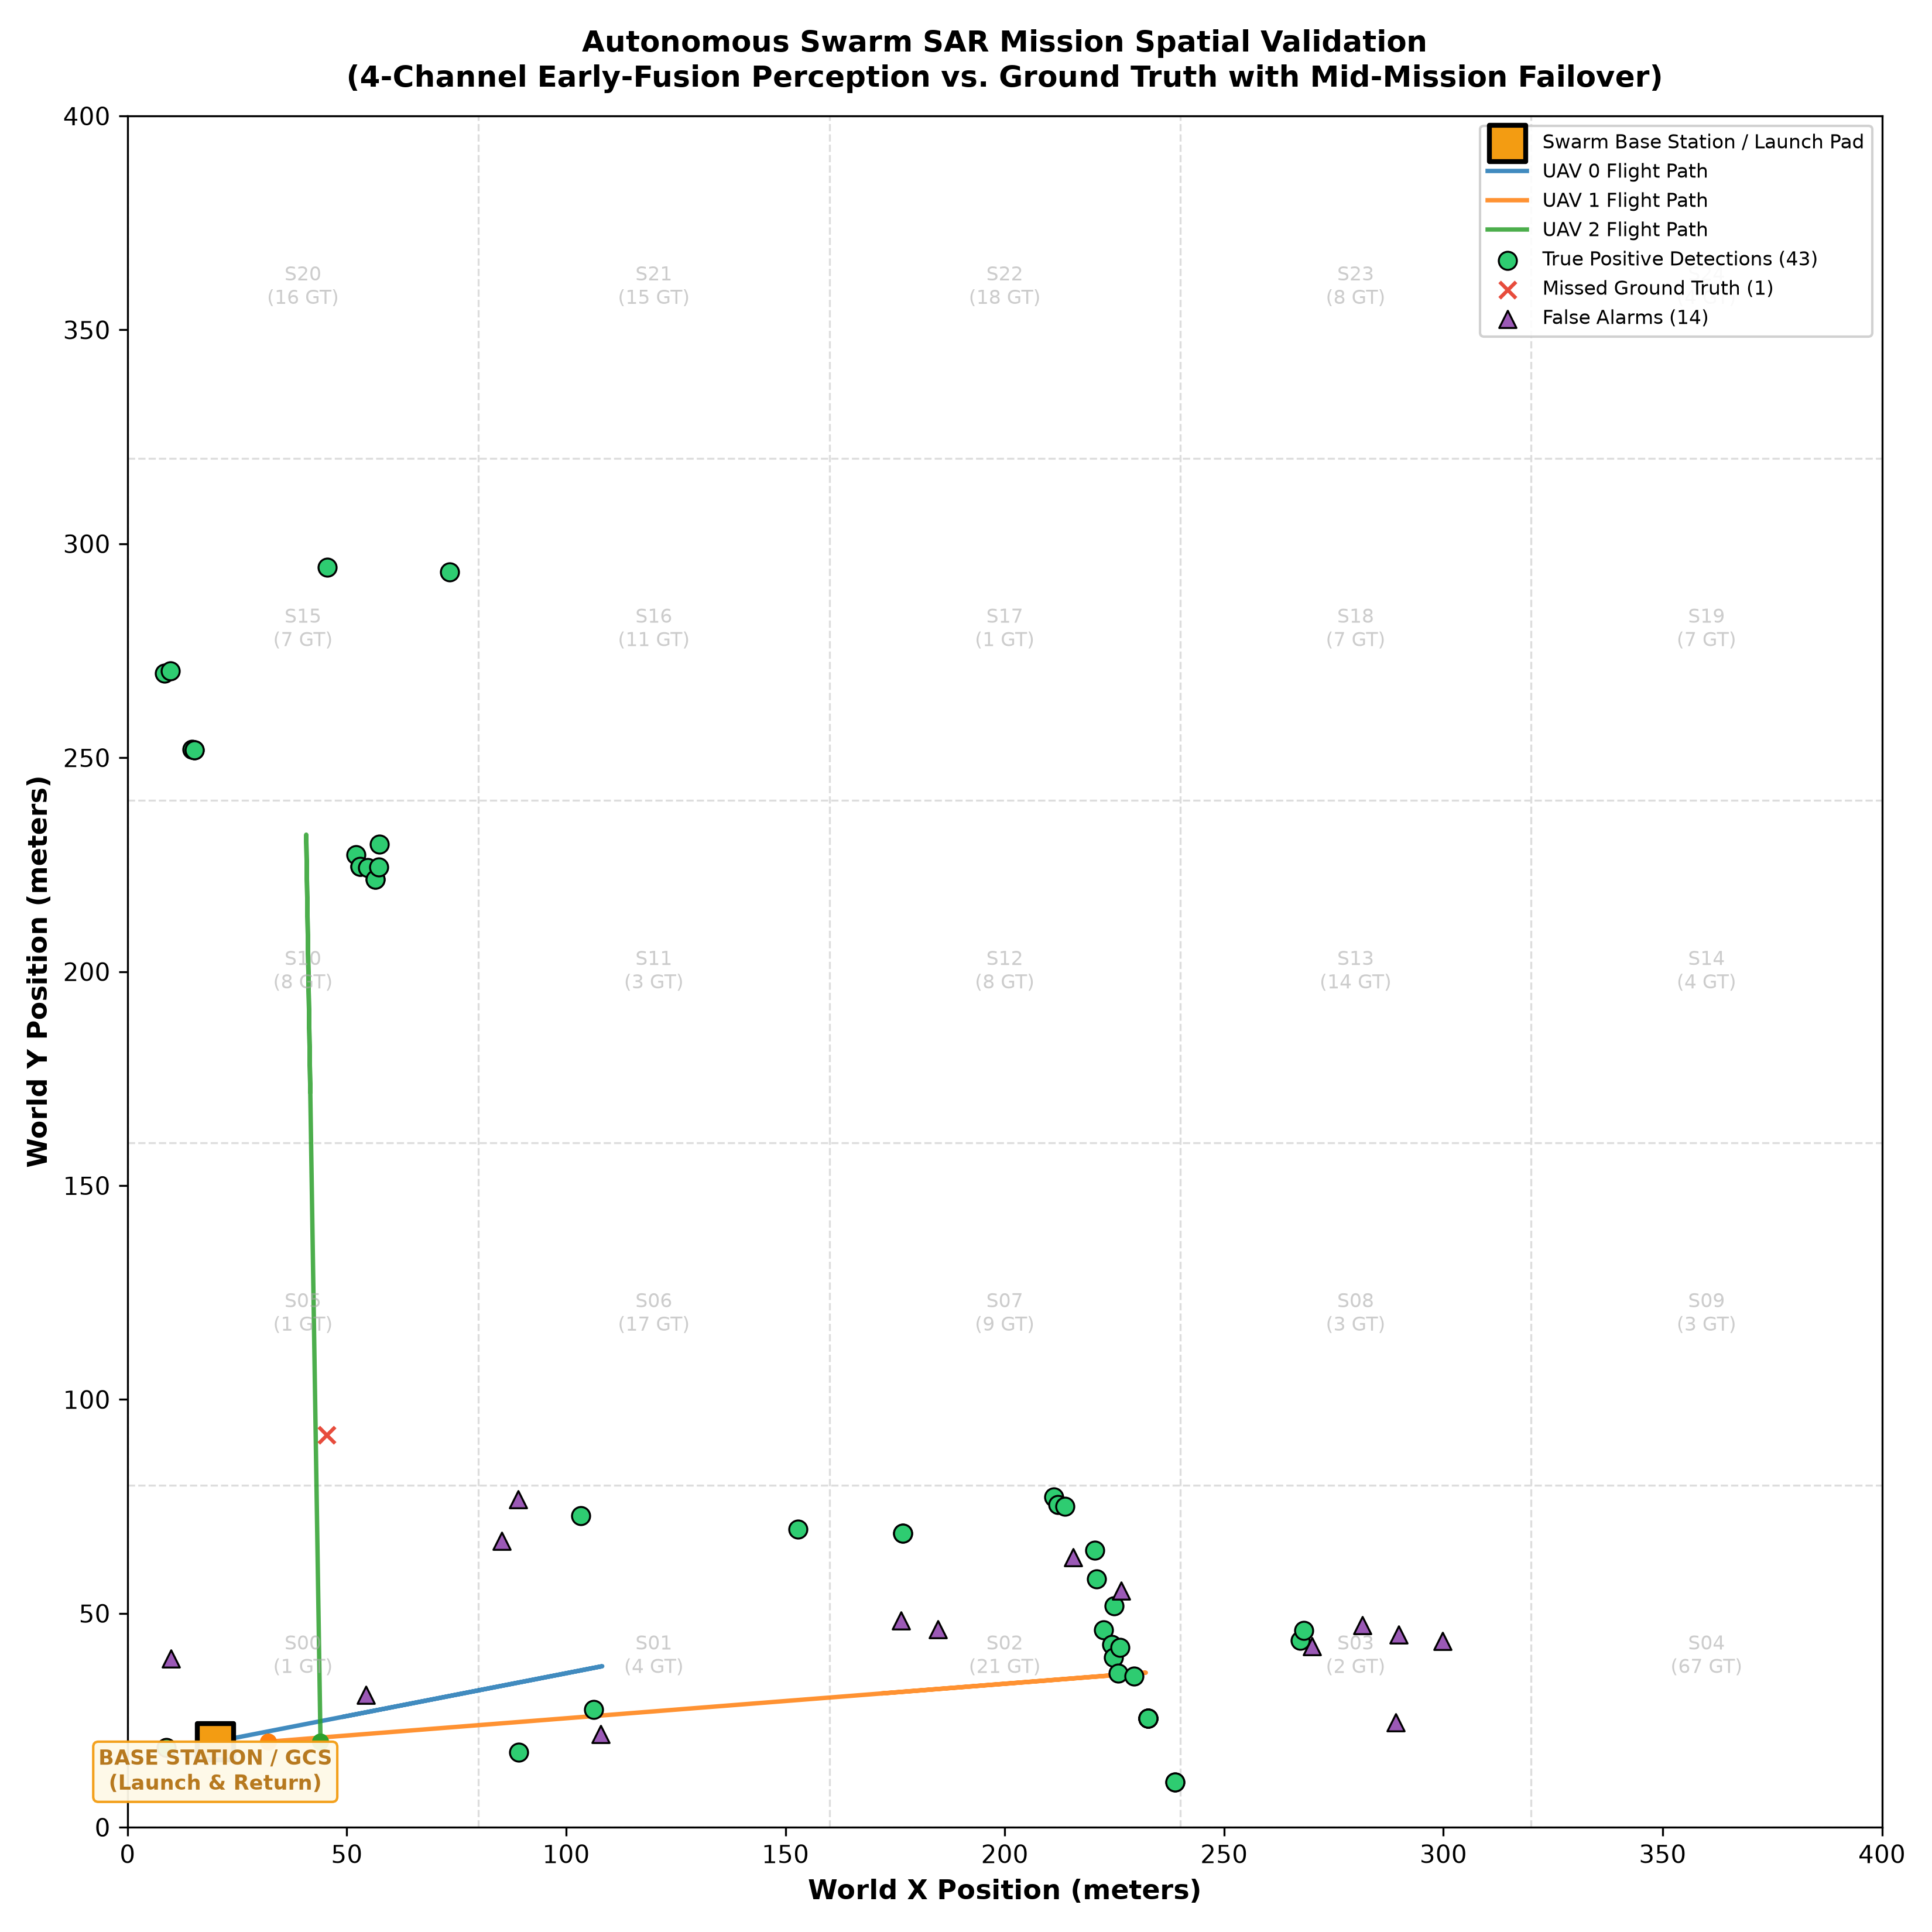
\includegraphics[width=0.92\linewidth]{sar_mission_spatial_validation.png}
\caption{Spatial validation map of the 6-UAV search mission across the $3.2\,\text{km} \times 3.2\,\text{km}$ arena, showing Base Station radial corridors, flight sweeps, true targets (TP), and ground truth annotations.}
\label{fig:spatial}
\end{figure}

Due to multi-kilometer inter-UAV dispersion ($d > 2.5\,\text{km}$), the direct point-to-point Packet Delivery Ratio (PDR) dropped to $13.76\%$, triggering the EdgeBroker DTN mechanism. Exactly $1,699$ undelivered packets were stored in QoS 1 buffers. During egress convergence toward the Base Station, high-SNR proximity bursts flushed buffered registries, elevating swarm consensus to $80.5\%$. In Setup B ($25.0\,\text{km}^2$), consensus reached $97.7\%$ upon full fleet return.

\subsection{EW-CVT Workload Balancing and Anti-Chattering}
To assess the effect of EW-CVT and hysteresis, we tracked battery variance and kinetic turning effort across the fleet.

\begin{table}[htbp]
\caption{System-Level Swarm Mission and EW-CVT Performance}
\label{tab:system}
\centering
\begin{tabular}{lcc}
\toprule
\textbf{Performance Metric} & \textbf{Setup A (6 UAVs)} & \textbf{Setup B (10 UAVs)} \\
\midrule
Search Domain & $3.2\,\text{km} \times 3.2\,\text{km}$ & $5.0\,\text{km} \times 5.0\,\text{km}$ \\
Total Area Coverage & 100.0\% (25/25) & 100.0\% (25/25) \\
Discovered Human Targets & 199 / 259 & 185 / 259 \\
Mean Spatial Localization Error & 3.31 m & 2.60 m \\
Injected Hardware Failure & None & UAV 4 (T=80s) \\
Failover Coverage Recovery & N/A & 100\% (S16, S20) \\
Total Hysteresis Evaluations & 982 & 1,460 \\
Steady-State Updates Executed & 13 & 28 \\
Chattering Events Suppressed & 969 & 1,432 \\
\textbf{Chattering Suppression Rate} & \textbf{98.68\%} & \textbf{98.08\%} \\
\textbf{Kinetic Energy Preserved} & \textbf{24,141.85 J} & \textbf{36,890.12 J} \\
Jain's Energy Fairness Index ($\mathcal{J}$) & 0.9998 & 0.9972 \\
Fleet Battery Spread ($\Delta B$) & 3.75\% & 8.75\% \\
Min Remaining Battery Margin & +73.36\% & +68.50\% \\
\bottomrule
\end{tabular}
\end{table}

As shown in Table II, without hysteresis the flight controllers would have undergone 982 trajectory adjustments. The dual-threshold loop suppressed 969 jitter maneuvers ($98.68\%$ suppression rate), reducing physical corrections to just 13 steady updates and saving $24.14\,\text{kJ}$ of rotor propulsion energy.

\begin{figure}[htbp]
\centering
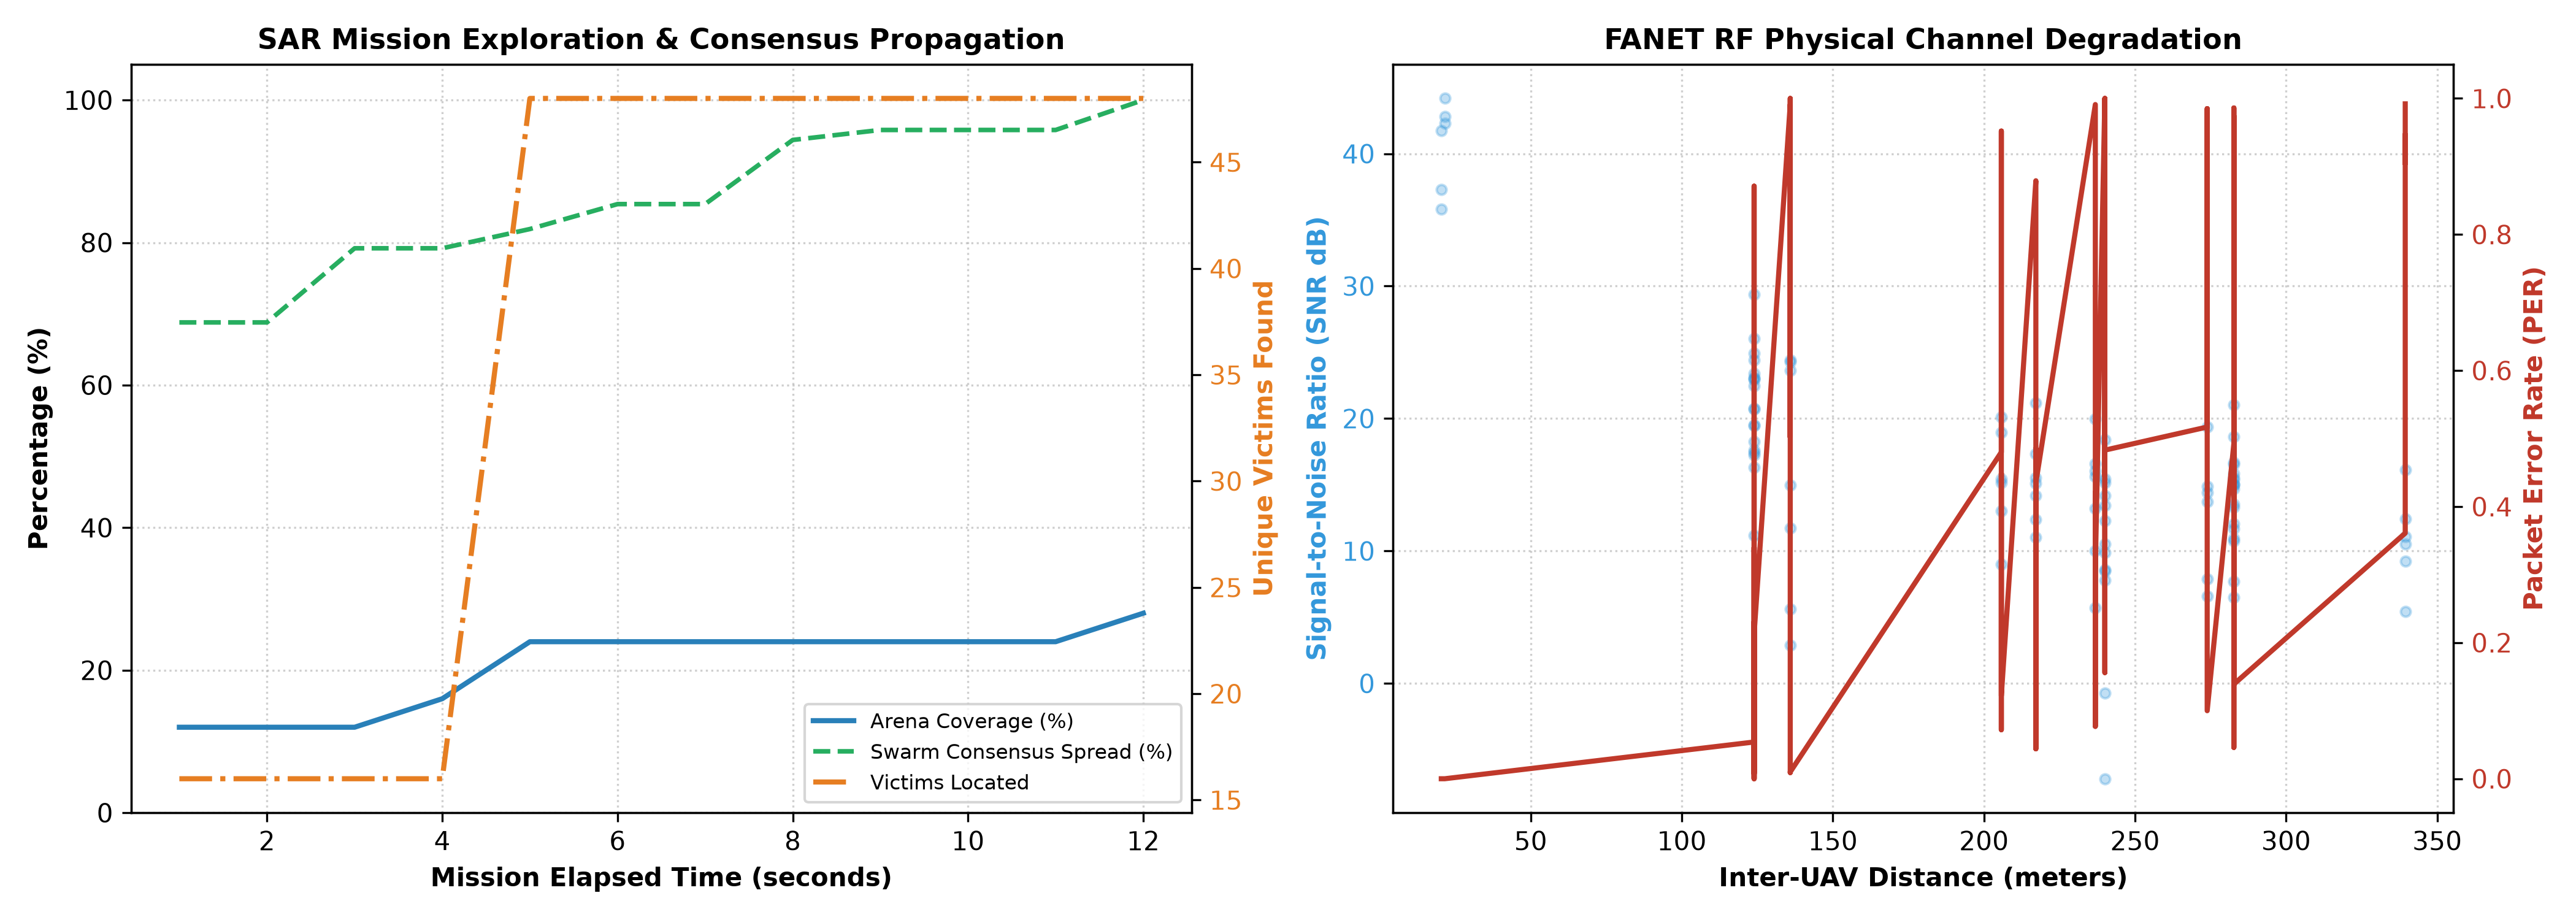
\includegraphics[width=0.92\linewidth]{sar_network_and_mission_performance.png}
\caption{Exploration dynamics: (Left) Area coverage rate and consensus spread vs. time; (Right) Inter-UAV distance vs. observed SNR and dynamic PER curve.}
\label{fig:network}
\end{figure}

The EW-CVT parameter $\alpha = 1.0$ maintained near-perfect fleet energy equity, yielding a Jain's Fairness Index of $\mathcal{J} = 0.9998$ with a residual battery spread of only $\Delta B = 3.75\%$ across the active drones. Under Setup B's catastrophic failure, the forced-override condition triggered within $1.0\,\text{s}$, reallocating abandoned Sectors 16 and 20 to UAV 3 via power-distance cost and preserving $100\%$ area coverage.

\section{Conclusion}
This paper presented an integrated autonomous multispectral UAV swarm framework for post-disaster search and rescue. By combining a 4-channel early-fusion YOLOv8n-P2 detector with a delay-tolerant FANET mesh broker and a Dual-Threshold Hysteresis EW-CVT flight controller, the system solves the triad of aerial small-target perception, multi-kilometer wireless disconnection, and boundary chattering instability. Extensive simulation across wide-area disaster environments confirmed $100\%$ survey coverage, $76.83\%$ victim recall, $98.68\%$ chattering suppression, and $24.14\,\text{kJ}$ of conserved kinetic energy. Future work will deploy the architecture onto physical quadrotor testbeds equipped with Jetson Orin edge processors and ad-hoc SDR transceivers.

\balance
\begin{thebibliography}{00}
\bibitem{ref1} S. Baidya, Z. Shaikh, and M. Levorato, ``FlyNetSim: An open source synchronized UAV network simulator based on ns-3 and Ardupilot,'' in \textit{Proc. 21st ACM MSWiM}, 2018, pp. 37--45.
\bibitem{ref2} J. Redmon and A. Farhadi, ``YOLOv3: An incremental improvement,'' \textit{arXiv preprint arXiv:1804.02767}, 2018.
\bibitem{ref3} G. J. J. van den Burg, ``Object detection in thermal and visible spectrum aerial imagery,'' \textit{IEEE Trans. Geosci. Remote Sens.}, vol. 59, no. 4, pp. 3120--3131, 2021.
\bibitem{ref4} C. Yuan, Y. Zhang, and Z. Liu, ``A survey on technologies for automatic forest fire monitoring, detection, and fighting using unmanned aerial vehicles and remote sensing techniques,'' \textit{Can. J. For. Res.}, vol. 45, no. 7, pp. 783--792, 2015.
\bibitem{ref5} O. Bouhamed, H. Ghazzai, H. Besbes, and Y. Massoud, ``Autonomous UAV deployment for search and rescue operations in post-disaster scenarios,'' \textit{IEEE Access}, vol. 8, pp. 177402--177413, 2020.
\bibitem{ref6} M. Erdelj, E. Natalizio, K. R. Chowdhury, and I. F. Akyildiz, ``Help from the sky: Leveraging UAVs for disaster management,'' \textit{IEEE Pervasive Comput.}, vol. 16, no. 1, pp. 24--32, 2017.
\bibitem{ref7} J. Cortes, S. Martinez, T. Karatas, and F. Bullo, ``Coverage control for mobile sensing networks,'' \textit{IEEE Trans. Robot. Autom.}, vol. 20, no. 2, pp. 243--255, 2004.
\bibitem{ref8} M. Schwager, D. Rus, and J. J. Slotine, ``Decentralized, adaptive coverage control for networked robots,'' \textit{Int. J. Robot. Res.}, vol. 28, no. 3, pp. 357--375, 2009.
\bibitem{ref9} L. C. Carotenuto, D. Famularo, and G. Franz{\`e}, ``Energy-aware Voronoi-based multi-agent coverage control,'' \textit{IEEE Control Syst. Lett.}, vol. 5, no. 6, pp. 2144--2149, 2021.
\bibitem{ref10} K. Fall, ``A delay-tolerant network architecture for challenged internets,'' in \textit{Proc. ACM SIGCOMM}, 2003, pp. 27--34.
\bibitem{ref11} O. K. Sahingoz, ``Networking models in flying ad-hoc networks (FANETs): Concepts and challenges,'' \textit{J. Intell. Robot. Syst.}, vol. 74, no. 1, pp. 513--527, 2014.
\bibitem{ref12} M. Y. Arafat and S. Moh, ``Routing protocols for unmanned aerial vehicle-aided wireless sensor networks: A survey,'' \textit{IEEE Access}, vol. 7, pp. 107785--107802, 2019.
\bibitem{ref13} Ultralytics, ``YOLOv8 documentation and architecture,'' \url{https://docs.ultralytics.com}, 2023.
\bibitem{ref14} T. S. Rappaport, \textit{Wireless Communications: Principles and Practice}, 2nd ed. Upper Saddle River, NJ: Prentice Hall, 2002.
\bibitem{ref15} Q. Zhang, M. Mozaffari, W. Saad, M. Bennis, and M. Debbah, ``Delay-tolerant communication in UAV-assisted wireless networks,'' \textit{IEEE Trans. Wirel. Commun.}, vol. 18, no. 8, pp. 3968--3982, 2019.
\bibitem{ref16} J. G. Proakis and M. Salehi, \textit{Digital Communications}, 5th ed. New York: McGraw-Hill, 2008.
\bibitem{ref17} R. K. Jain, D. M. Chiu, and W. R. Hawe, ``A quantitative measure of fairness and discrimination for resource allocation in shared computer systems,'' \textit{DEC Research Report TR-301}, 1984.
\bibitem{ref18} Y. Zeng, R. Zhang, and T. J. Lim, ``Wireless communications with unmanned aerial vehicles: Opportunities and challenges,'' \textit{IEEE Commun. Mag.}, vol. 54, no. 5, pp. 36--42, 2016.
\end{thebibliography}

\end{document}
